\clearpage
\section{Quiz Statistics} 
\hspace{0.5cm} 
    
   
\subsection{Problem statement}
	Create a statistics page per quiz that shows the following statistics
	\begin{enumerate}
	    \item Shows mark distribution of the quiz as a Cumulative Distributive Function (CDF)
	    \item Show the statistics per question of number of students who have answers the question correctly, incorrectly and did not attempt.
		\item Show top 5 answers per questions and the percentage of students who chose each option
		\item General stats about the quiz such as total number of students, total number of submissions, average marks, total marks
	\end{enumerate}

\subsection{Why do we need this?}
	One of the advantages of conducting in class quizzes using the SAFE platform is the immediate feedback. The instructor can know the performance of the students as soon as the quiz is over. The above mentioned statistics will aid the instructor in judging the overall performance of the students, as well as any questions which the students found particularly difficult, so that more time can be spent on the topics in which the student performance was low 

\subsection{Design}
	Ideally the statistics should be calculated when the quiz ends. But since the old version of SAFE did not have a job subsystem which tracks if the particular quiz has ended or not, we have to calculate the statistics each time the statistics page is loaded. We cache the calculated statistics to avoid re-computation if the quiz is not changed the next time the page is loaded. In the new version of SAFE we have an asynchronous task runner using Celery which takes care of problem, and statistics can be calculated when the quiz ends.

\subsection{Implementation}
	The statistics are calculated by iterating over all the submissions for the given quiz. The format of the submission and different question types are given in the table

	The logic for calculating different statistics values are as follows

    \begin{enumerate}    
        \item  \textbf{CDF} - Dictionary with key as floor of marks and value as the count of students who have obtained that mark
	    \item  \textbf{Average Marks} - Calculate sum of marks while iterating through the submissions and take average
	    \item  \textbf{Question Stats} - For each question (response) inside a submission increment the count of the corresponding question depending on whether its correct, wrong or not answered	
	    \item  \textbf{Answer Statistics}
	    \begin{itemize}
	        \item For Single Correct answer question we maintain the count of students who chose each option
		    \item For other question types we find the top 5 answers and their counts using priority queue with a comma concatenated string of answers (in case of multiple answers) as the key and the count as the priority
		\end{itemize}
	\end{enumerate}

	Once the statistics are calculated we save it into the statistics table. This table has a field which stores the timestamp of when the quiz is evaluated when the stats were last calculated. This enables to check if the quiz has been modified and if the statistics needs to be recalculated
	
	On the frontend side the graphs are drawn using morris chart javascript chart library

    \begin{center}
    Listing 1 : Representation of different types of questions
    \end{center}
	
    \inputminted{json}{code/question-type.json}

\subsection{Screenshots}
    \begin{figure}[h!]
    \begin{center}
    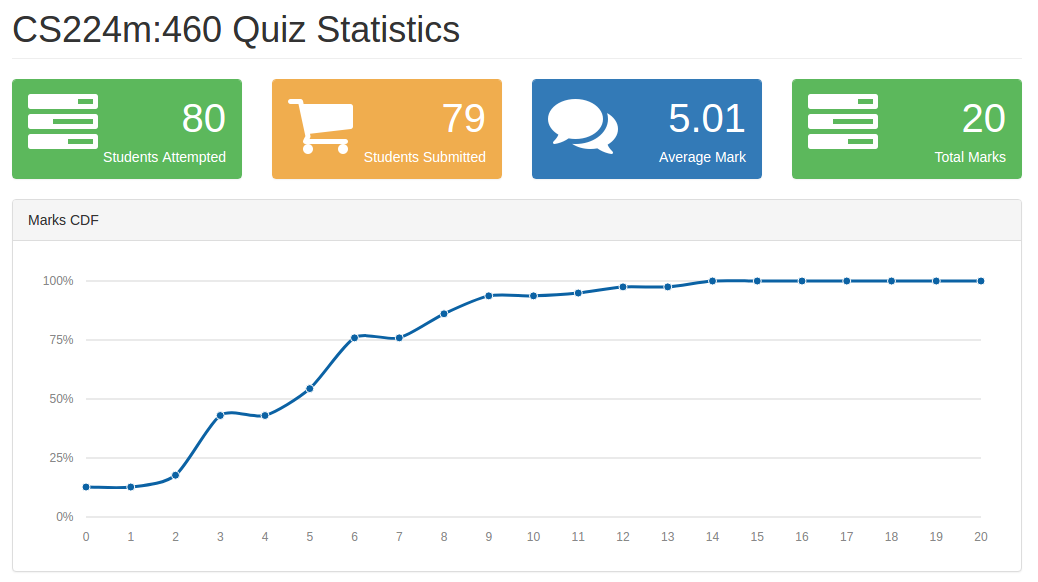
\includegraphics[scale=.4]{diagrams/quiz_stat_1.png} 
    \vspace{1cm}
    \caption{Quiz Statistics Page}
    \end{center}
    \end{figure}
    
    \begin{figure}[h!]
    \begin{center}
    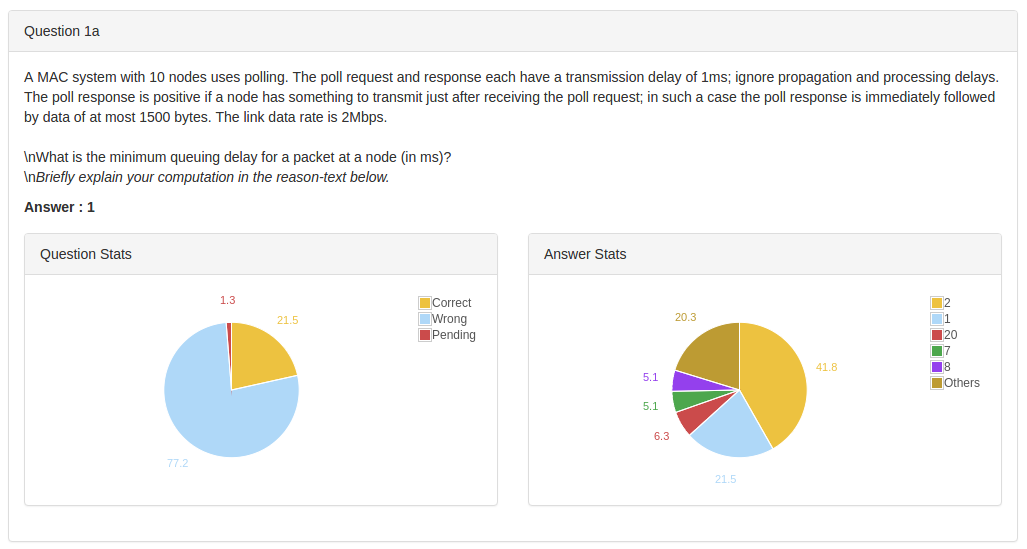
\includegraphics[scale=.4]{diagrams/quiz-stat-2.png} 
    \vspace{1cm}
    \caption{Question statistics}
    \end{center}
    \end{figure}